%! Unidad 4 — Interacción gravitatoria (teoría, actividades resueltas y prácticas)
%! Fuente: Fuentes/Tema_4.pdf (reescrito; datos de las actividades cambiados y recalculados)

\section*{Para empezar: la manzana y la Luna}
\addcontentsline{toc}{section}{Para empezar: la manzana y la Luna}

Cuenta la leyenda que Isaac Newton, viendo caer una manzana, se preguntó si la fuerza que la hacía caer era la misma que
mantenía a la Luna girando alrededor de la Tierra. Hizo la cuenta: la Luna está unas 60 veces más lejos del centro de la
Tierra que la manzana, y su aceleración hacia la Tierra resulta ser unas \(60^2 = 3600\) veces menor que \(g\). Era la misma
fuerza, debilitada con el cuadrado de la distancia. Con esa idea unificó por primera vez la física «de la Tierra» y la «del
cielo». En esta unidad recorreremos ese camino: desde las leyes de Kepler hasta la ley de la gravitación universal, el
concepto de campo y el movimiento de planetas y satélites.

\section{Modelos del universo}\label{sec:grav-modelos}

\paragraph{Modelos geocéntricos.} En la Antigüedad se pensaba que la Tierra estaba inmóvil en el centro del universo y que
todos los astros, también el Sol, giraban a su alrededor. Para \textbf{Aristóteles} (siglo \textsc{iv} a.\,C.) el universo
tenía dos regiones: la \emph{sublunar}, formada por los cuatro elementos (tierra, agua, aire y fuego), donde todo cambia, y
la \emph{celeste}, donde los astros se movían en esferas concéntricas con movimientos circulares, uniformes y eternos.

\textbf{Ptolomeo} (siglo \textsc{ii}) perfeccionó el modelo para explicar que los planetas a veces parecen retroceder en el
cielo: cada planeta gira en un círculo pequeño, el \azuln{epiciclo}, cuyo centro gira a su vez alrededor de la Tierra en un
círculo mayor, el \azuln{deferente} (figura~\ref{fig:grav-modelos}). Este modelo se usó durante casi 1500 años.

\paragraph{Modelos heliocéntricos.} En 1543 \textbf{Copérnico} propuso que el Sol está en el centro y que la Tierra es un
planeta más, que gira sobre sí misma y alrededor del Sol. La idea chocaba con la interpretación de la época de las Sagradas
Escrituras y tardó en aceptarse. \textbf{Galileo} la defendió con las observaciones de su telescopio (las lunas de Júpiter,
las fases de Venus), lo que le costó un proceso de la Inquisición en 1633. Las medidas muy precisas del danés
\textbf{Tycho Brahe} permitieron a su ayudante \textbf{Kepler} enunciar las leyes del movimiento planetario, y con ellas el
modelo heliocéntrico quedó establecido.

\begin{figure}[H]
    \centering
    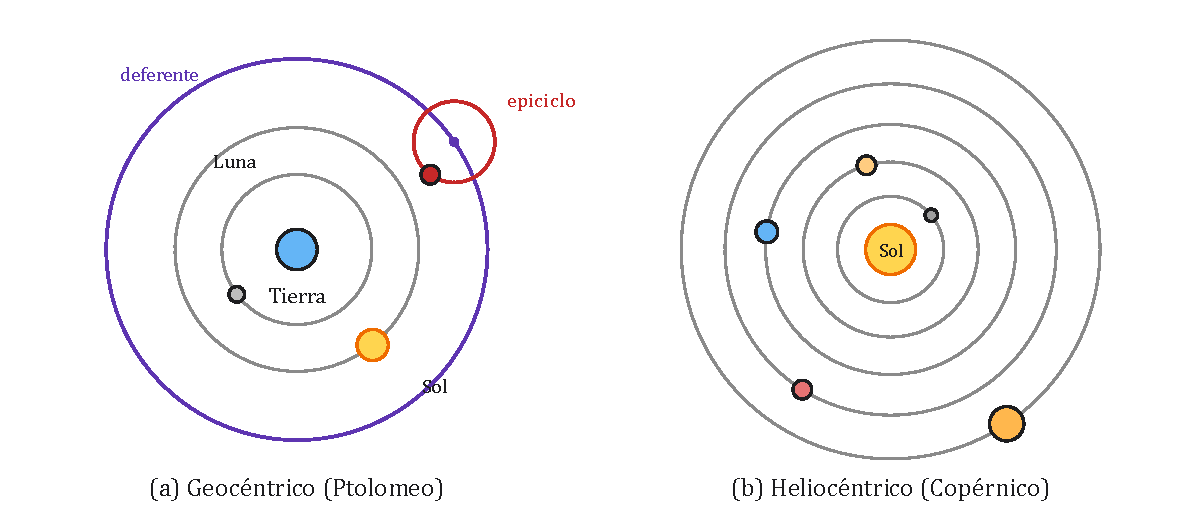
\includegraphics[width=0.88\linewidth]{images/UD4/modelos}
    \caption{(a) En el modelo de Ptolomeo, Marte gira en un epiciclo cuyo centro recorre el deferente alrededor de la Tierra.
    (b) En el de Copérnico, los planetas giran alrededor del Sol.}
    \label{fig:grav-modelos}
\end{figure}

\section{Las leyes de Kepler}\label{sec:grav-kepler}

Kepler dedicó años a analizar las observaciones de Brahe sobre Marte y llegó a tres leyes \emph{empíricas} (deducidas de
los datos, sin explicar su causa):

\begin{definition}[Leyes de Kepler]
    \begin{enumerate}[label=\numberballmDarkTeal]
        \item \rojon{Ley de las órbitas}. Los planetas describen órbitas elípticas, con el Sol en uno de sus focos.
        \item \rojon{Ley de las áreas}. El radio vector que une el Sol con un planeta barre áreas iguales en tiempos iguales:
        la \azuln{velocidad areolar} \(dA/dt\) es constante.
        \item \rojon{Ley de los períodos}. Los cuadrados de los períodos de revolución son proporcionales a los cubos de los
        semiejes mayores de las órbitas (o de los radios medios):
        \begin{centeredequation}
            \boxed{\dfrac{T^2}{r^3} = \text{constante}} \qquad\Rightarrow\qquad \dfrac{T_1^2}{r_1^3} = \dfrac{T_2^2}{r_2^3} \label{eq:grav-kepler3}
        \end{centeredequation}
    \end{enumerate}
\end{definition}

\begin{figure}[H]
    \centering
    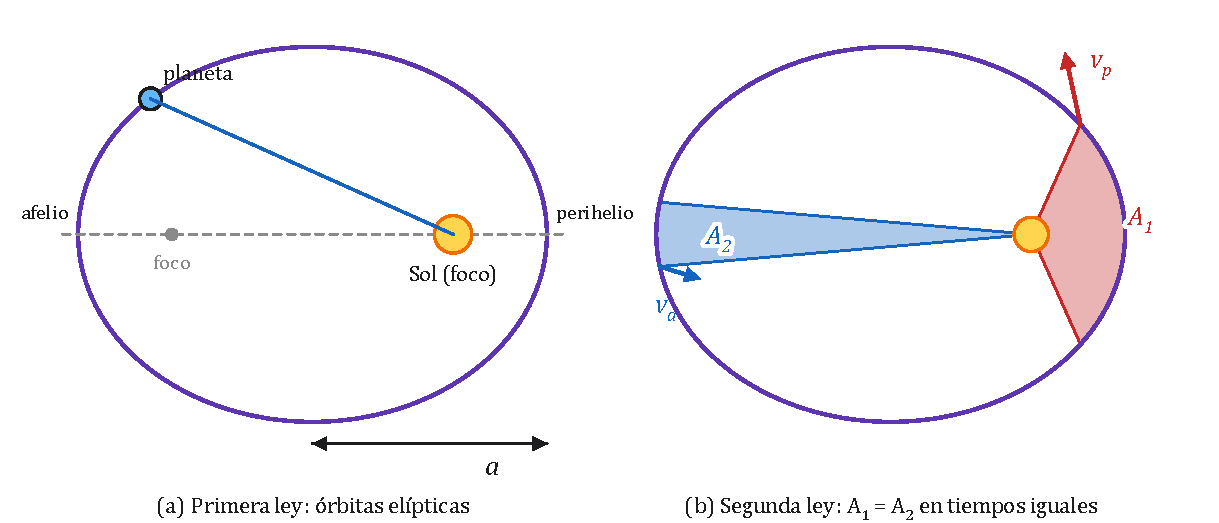
\includegraphics[width=0.95\linewidth]{images/UD4/kepler}
    \caption{(a) Órbita elíptica (muy exagerada: las órbitas de los planetas son casi circulares). (b) Las dos zonas
    sombreadas se barren en el mismo tiempo: cerca del Sol el planeta va más deprisa.}
    \label{fig:grav-kepler}
\end{figure}

El punto de la órbita más cercano al Sol es el \azuln{perihelio} y el más lejano, el \azuln{afelio} (para la Tierra,
\emph{perigeo} y \emph{apogeo}). Las tres leyes valen también para cualquier conjunto de satélites que giran alrededor de un
mismo astro central (las lunas de Júpiter, los satélites artificiales de la Tierra), pero con una constante distinta en la
tercera ley para cada astro central.

\begin{exercise}
    Ío, una de las lunas de Júpiter, gira en una órbita de \qty{4.22e5}{\km} de radio con un período de \qty{1.77}{días}.
    Europa gira a \qty{6.71e5}{\km}. ¿Cuál es el período de Europa?
    \begin{solu}
        \textcolor{blue}{Las dos giran alrededor de Júpiter: misma constante en la tercera ley.}
        \[ T_E = T_I\left(\dfrac{r_E}{r_I}\right)^{3/2} = 1{,}77\left(\dfrac{6{,}71}{4{,}22}\right)^{3/2} = \textcolor{red}{\qty{3.55}{días}} \]
    \end{solu}
\end{exercise}

\section{Momento angular}\label{sec:grav-momento}

Para justificar las dos primeras leyes de Kepler necesitamos una nueva magnitud.

\begin{definition}[Momento angular]
    El \rojon{momento angular} (o cinético) de una partícula de masa \(m\) y velocidad \(\vec v\) respecto de un punto \(O\) es:
    \begin{centeredequation}
        \boxed{\vec L = \vec r \times \vec p = \vec r \times m\vec v} \label{eq:grav-L}
    \end{centeredequation}
    donde \(\vec r\) es el vector de posición de la partícula respecto de \(O\). Se mide en \unit{\kg\m\squared\per\second}.
\end{definition}

Por ser un producto vectorial, \(\vec L\) es perpendicular al plano que forman \(\vec r\) y \(\vec v\); su sentido es el de
avance de un sacacorchos que gira llevando \(\vec r\) hacia \(\vec v\) por el camino más corto, y su módulo es
\(L = r\,m\,v\sen\varphi\) (figura~\ref{fig:grav-L}).

\begin{figure}[H]
    \centering
    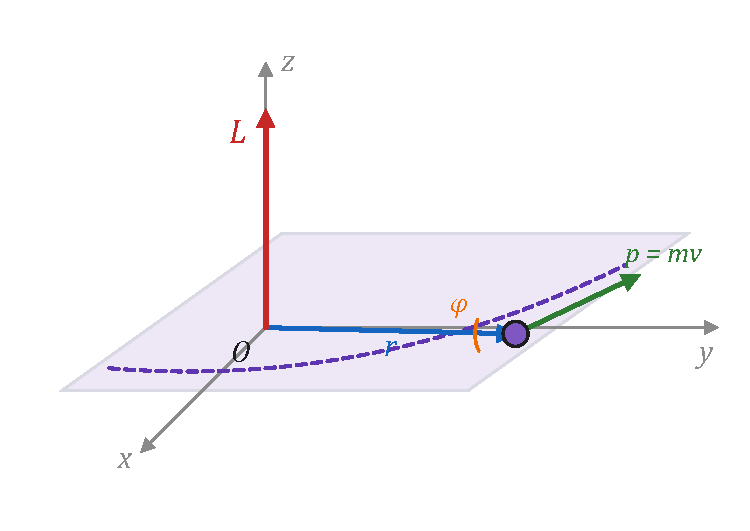
\includegraphics[width=0.48\linewidth]{images/UD4/momento_angular}
    \caption{El momento angular es perpendicular al plano en el que se mueve la partícula.}
    \label{fig:grav-L}
\end{figure}

\paragraph{Conservación del momento angular.} Derivando respecto del tiempo:
\begin{equation*}
    \dfrac{d\vec L}{dt} = \dfrac{d\vec r}{dt}\times m\vec v + \vec r\times\dfrac{d(m\vec v)}{dt} = \underbrace{\vec v\times m\vec v}_{0} + \vec r\times\vec F = \vec M
\end{equation*}
El primer término es nulo porque los dos vectores son paralelos; el segundo es el \azuln{momento de la fuerza}
\(\vec M = \vec r\times\vec F\).
\begin{remark}
    Si el momento de la fuerza que actúa sobre una partícula respecto de un punto es nulo, el momento angular respecto de ese
    punto \textbf{se conserva} (es constante en módulo, dirección y sentido).
\end{remark}

\paragraph{Fuerzas centrales.} Una fuerza es \rojon{central} si está siempre dirigida hacia un mismo punto, el
\emph{centro de fuerzas}. La atracción del Sol sobre un planeta es central. Como \(\vec F\) es paralela a \(\vec r\),
\(\vec M = \vec r \times\vec F = 0\): \textbf{bajo una fuerza central el momento angular se conserva}.

\paragraph{Justificación de las dos primeras leyes de Kepler.}
\begin{itemize}
    \item Como \(\vec L\) tiene dirección constante y es perpendicular a \(\vec r\) y \(\vec v\), el planeta se mueve
    siempre en el mismo plano: la órbita es una \textbf{curva plana} (Newton demostró después que es una elipse).
    \item En un tiempo \(dt\) el radio vector barre un triángulo de área \(dA = \frac{1}{2}\,r\,v\,dt\sen\varphi\). Como
    \(L = r\,m\,v\sen\varphi\):
    \begin{centeredequation}
        \dfrac{dA}{dt} = \dfrac{1}{2}\,r\,v\sen\varphi = \boxed{\dfrac{L}{2m}} = \text{constante} \label{eq:grav-areolar}
    \end{centeredequation}
    la velocidad areolar es constante: es la segunda ley.
\end{itemize}
En el perihelio y en el afelio la velocidad es perpendicular al radio vector (\(\sen\varphi = 1\)), y la conservación de
\(L\) da \(m\,r_p v_p = m\,r_a v_a\), es decir:
\begin{centeredequation}
    \boxed{r_p\,v_p = r_a\,v_a} \label{eq:grav-perihelio}
\end{centeredequation}
El planeta va más deprisa en el perihelio. En una órbita circular la velocidad es constante (movimiento uniforme).

\begin{exercise}
    Un satélite de \qty{1500}{\kg} describe una órbita elíptica alrededor de la Tierra. En el perigeo está a \qty{400}{\km}
    de altura y lleva una velocidad de \qty{8071}{\m\per\second}; en el apogeo está a \qty{2000}{\km} de altura
    (\(R_T = \qty{6370}{\km}\)). Calcula su momento angular respecto del centro de la Tierra y su velocidad en el apogeo.
    \begin{solu}
        \textcolor{blue}{Distancias al centro: \(r_p = \qty{6.77e6}{\m}\), \(r_a = \qty{8.37e6}{\m}\).}

        \(L = m\,r_p v_p = 1500\cdot 6{,}77\cdot 10^6\cdot 8071 = \textcolor{red}{\qty{8.20e13}{\kg\m\squared\per\second}}\).

        \(v_a = \dfrac{r_p v_p}{r_a} = \dfrac{6{,}77\cdot 8071}{8{,}37} = \textcolor{red}{\qty{6528}{\m\per\second}}\).
    \end{solu}
\end{exercise}

\begin{exercise}
    Calcula la velocidad areolar de la Tierra alrededor del Sol suponiendo su órbita circular de \qty{1.496e11}{\m} de radio.
    \begin{solu}
        \textcolor{blue}{En un año barre el círculo entero:}
        \(\dfrac{dA}{dt} = \dfrac{\pi r^2}{T} = \dfrac{\pi (1{,}496\cdot 10^{11})^2}{3{,}156\cdot 10^7} = \textcolor{red}{\qty{2.23e15}{\m\squared\per\second}}\).
    \end{solu}
\end{exercise}

\section{Ley de la gravitación universal}\label{sec:grav-newton}

\subsection{Deducción a partir de las leyes de Kepler}\label{subsec:grav-deduccion}

Supongamos órbitas circulares (para casi todos los planetas es una aproximación excelente: la órbita de la Tierra tiene un
cociente entre semiejes de \num{0.9998}). Por la segunda ley, el movimiento es uniforme, \(v = 2\pi r/T\), y la aceleración
del planeta es la centrípeta:
\begin{equation*}
    a = \dfrac{v^2}{r} = \dfrac{4\pi^2 r}{T^2} = \dfrac{4\pi^2}{r^2}\cdot\dfrac{r^3}{T^2}
\end{equation*}
Por la tercera ley, \(r^3/T^2\) es la misma constante para todos los planetas: la aceleración es inversamente proporcional al
cuadrado de la distancia, y la fuerza que la produce también, \(F = m\,a \propto m/r^2\). Por la tercera ley de Newton, la
fuerza que el planeta ejerce sobre el Sol es igual y opuesta, así que también debe ser proporcional a la masa del Sol.

\subsection{Enunciado}\label{subsec:grav-enunciado}

\begin{definition}[Ley de la gravitación universal]
    Dos cuerpos cualesquiera se atraen con una fuerza directamente proporcional al producto de sus masas e inversamente
    proporcional al cuadrado de la distancia entre sus centros:
    \begin{centeredequation}
        \boxed{\vec F_{12} = -\,G\,\dfrac{m_1 m_2}{r^2}\,\vec u_r} \qquad\qquad F = G\,\dfrac{m_1 m_2}{r^2} \label{eq:grav-newton}
    \end{centeredequation}
    donde \(\vec u_r\) es un vector unitario que va de la masa que ejerce la fuerza a la que la sufre (el signo menos indica
    atracción) y \(G = \qty{6.67e-11}{\newton\m\squared\per\kg\squared}\) es la \azuln{constante de gravitación universal}.
\end{definition}

\begin{figure}[H]
    \centering
    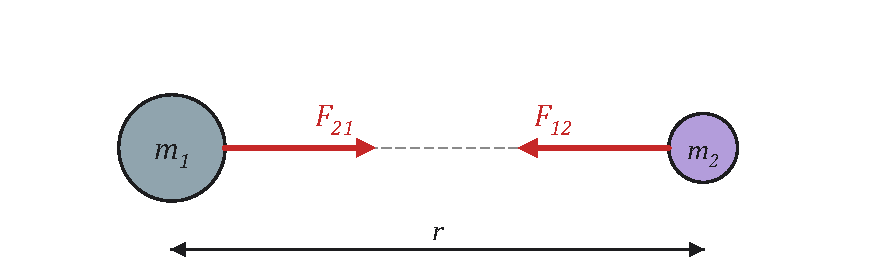
\includegraphics[width=0.6\linewidth]{images/UD4/gravitacion}
    \caption{Las fuerzas con que se atraen dos masas son iguales en módulo, de sentidos opuestos y están sobre la recta que
    une sus centros.}
    \label{fig:grav-fuerza}
\end{figure}

\begin{remark}
    \(G\) es la fuerza con que se atraen dos masas de \qty{1}{\kg} separadas \qty{1}{\m}. Su valor es tan pequeño que la
    atracción entre objetos cotidianos es imperceptible; solo se nota cuando al menos uno de los cuerpos tiene una masa
    enorme. Cavendish lo midió por primera vez en 1798 con una balanza de torsión, lo que permitió «pesar la Tierra».
\end{remark}

\paragraph{Principio de superposición.} Si sobre una masa actúan varias, la fuerza total es la suma vectorial de las
fuerzas que ejerce cada una por separado: \(\vec F = \vec F_1 + \vec F_2 + \vec F_3 + \cdots\) Para calcularla se escogen unos
ejes, se descompone cada fuerza en componentes \(\vec F = F_x\,\vec{i} + F_y\,\vec{j}\) y se suman.

\begin{exercise}
    Tres masas de \qty{2}{\kg}, \qty{5}{\kg} y \qty{6}{\kg} están en los puntos \((0, 0)\), \((0, 4)\) y \((3, 0)\),
    respectivamente (distancias en metros). Calcula la fuerza gravitatoria sobre la masa del origen.
    \begin{solu}
        \textcolor{blue}{La de \qty{5}{\kg} la atrae hacia \(+Y\) y la de \qty{6}{\kg} hacia \(+X\):}
        \[ \vec F_5 = G\,\dfrac{5\cdot 2}{4^2}\,\vec{j} = 4{,}17\cdot 10^{-11}\,\vec{j}\ \unit{\newton} \qquad
           \vec F_6 = G\,\dfrac{6\cdot 2}{3^2}\,\vec{i} = 8{,}89\cdot 10^{-11}\,\vec{i}\ \unit{\newton} \]
        \(\textcolor{red}{\vec F = (8{,}89\,\vec{i} + 4{,}17\,\vec{j})\cdot 10^{-11}\ \unit{\newton}}\);
        \(F = \textcolor{red}{\qty{9.82e-11}{\newton}}\), \textcolor{red}{a \ang{25.1} del eje \(X\)}.
    \end{solu}
\end{exercise}

\begin{exercise}
    En tres vértices de un cuadrado de \qty{1.5}{\m} de lado hay masas de \qty{5}{\kg}. Calcula la fuerza sobre una masa de
    \qty{3}{\kg} situada en el cuarto vértice.
    \begin{solu}
        \textcolor{blue}{Pongamos la masa de \qty{3}{\kg} en el origen y las otras en \((1{,}5;\,0)\), \((0;\,1{,}5)\) y
        \((1{,}5;\,1{,}5)\). Las dos de los lados ejercen \(F_1 = G\,\dfrac{5\cdot 3}{1{,}5^2} = \qty{4.45e-10}{\newton}\) cada una;
        la de la diagonal, a \(1{,}5\sqrt 2\ \unit{\m}\), \(F_2 = G\,\dfrac{15}{4{,}5} = \qty{2.22e-10}{\newton}\), a \ang{45}.}
        \[ F_x = F_y = 4{,}45\cdot 10^{-10} + 2{,}22\cdot 10^{-10}\cos\ang{45} = \qty{6.02e-10}{\newton} \]
        \(\textcolor{red}{\vec F = 6{,}02\cdot 10^{-10}\,(\vec{i} + \vec{j})\ \unit{\newton}}\); \(F = \textcolor{red}{\qty{8.51e-10}{\newton}}\),
        \textcolor{red}{dirigida hacia el vértice opuesto.}
    \end{solu}
\end{exercise}

\subsection{La tercera ley de Kepler a partir de la ley de Newton}\label{subsec:grav-kepler3}

Para un planeta de masa \(m\) en órbita circular de radio \(r\) alrededor del Sol, la fuerza gravitatoria es la fuerza
centrípeta:
\begin{equation*}
    G\,\dfrac{M_S\,m}{r^2} = m\,\dfrac{v^2}{r} \;\Rightarrow\; v^2 = \dfrac{G M_S}{r} \qquad\text{y con } v = \dfrac{2\pi r}{T}:\qquad
    \dfrac{4\pi^2 r^2}{T^2} = \dfrac{G M_S}{r}
\end{equation*}
\begin{centeredequation}
    \boxed{\dfrac{T^2}{r^3} = \dfrac{4\pi^2}{G M}} \label{eq:grav-kepler3-newton}
\end{centeredequation}
La constante de la tercera ley solo depende de la masa del astro central \(M\). Midiendo el período y el radio de la órbita
de un satélite se puede calcular la masa del astro alrededor del que gira.

\section{El campo gravitatorio}\label{sec:grav-campo}

\subsection{El concepto de campo}\label{subsec:grav-concepto-campo}

Un \rojon{campo} es una región del espacio en la que a cada punto le corresponde un valor de una magnitud física. Si la
magnitud es escalar (la temperatura de una habitación), el campo es escalar; si es vectorial (la fuerza sobre una masa),
es vectorial. La idea de campo sustituye a la «acción a distancia»: una masa modifica el espacio que la rodea, y otra masa
colocada en él nota esa modificación.

Un campo vectorial se representa con \azuln{líneas de campo}: líneas tangentes en cada punto al vector del campo, dibujadas
de forma que su densidad sea proporcional a su módulo. Dos líneas de campo nunca se cortan (en el punto de corte el campo
tendría dos valores).

\subsection{Intensidad del campo gravitatorio}\label{subsec:grav-intensidad}

\begin{definition}[Intensidad del campo gravitatorio]
    La \rojon{intensidad del campo gravitatorio} \(\vec g\) en un punto es la fuerza que actuaría sobre la unidad de masa
    colocada en él: \(\vec g = \vec F/m\). Para el campo creado por una masa puntual (o esférica) \(M\) a una distancia \(r\):
    \begin{centeredequation}
        \boxed{\vec g = -\,G\,\dfrac{M}{r^2}\,\vec u_r} \qquad\qquad g = G\,\dfrac{M}{r^2} \label{eq:grav-g}
    \end{centeredequation}
    Se mide en \unit{\newton\per\kg} (equivalente a \unit{\m\per\second\squared}). Está dirigido hacia la masa que crea el campo.
\end{definition}

Conocido el campo, la fuerza sobre cualquier masa \(m\) es \(\vec F = m\,\vec g\). Si hay varias masas, el campo total es
la suma vectorial de los campos de cada una (\azuln{principio de superposición}, figura~\ref{fig:grav-superposicion}).

\begin{figure}[H]
    \centering
    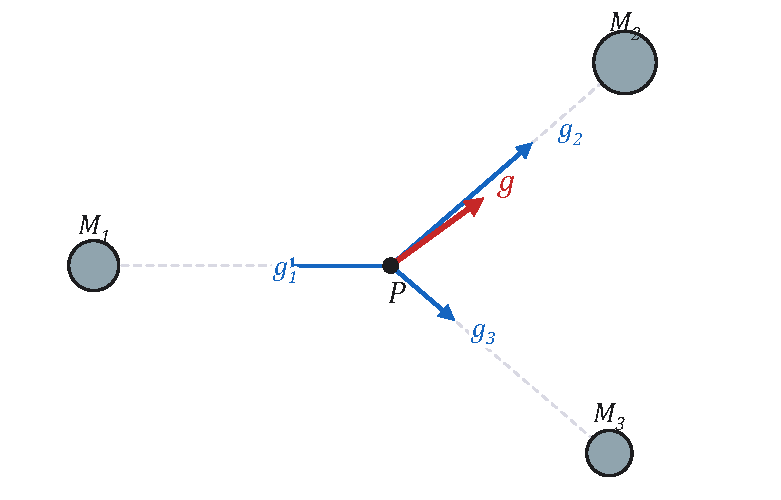
\includegraphics[width=0.5\linewidth]{images/UD4/superposicion}
    \caption{Cada masa crea en \(P\) un campo dirigido hacia ella. El campo total es la suma vectorial.}
    \label{fig:grav-superposicion}
\end{figure}

\begin{exercise}
    Calcula el campo gravitatorio en el punto \(P(4, 3)\) creado por tres masas de \qty{8}{\kg}, \qty{6}{\kg} y \qty{3}{\kg}
    situadas en \((0, 0)\), \((4, 0)\) y \((0, 3)\), respectivamente (distancias en metros).
    \begin{solu}
        \begin{itemize}
            \item \qty{8}{\kg}, a \qty{5}{\m}: \(g_1 = G\,\dfrac{8}{25} = \qty{2.13e-11}{\newton\per\kg}\), dirigido hacia el origen,
            \(\vec u = (-0{,}8;\,-0{,}6)\): \(\vec g_1 = (-1{,}71\,\vec{i} - 1{,}28\,\vec{j})\cdot 10^{-11}\).
            \item \qty{6}{\kg}, a \qty{3}{\m} por debajo: \(\vec g_2 = -G\,\dfrac{6}{9}\,\vec{j} = -4{,}45\cdot 10^{-11}\,\vec{j}\).
            \item \qty{3}{\kg}, a \qty{4}{\m} a la izquierda: \(\vec g_3 = -G\,\dfrac{3}{16}\,\vec{i} = -1{,}25\cdot 10^{-11}\,\vec{i}\).
        \end{itemize}
        \(\textcolor{red}{\vec g = (-2{,}96\,\vec{i} - 5{,}73\,\vec{j})\cdot 10^{-11}\ \unit{\newton\per\kg}}\); \(g = \textcolor{red}{\qty{6.45e-11}{\newton\per\kg}}\).
    \end{solu}
\end{exercise}

\subsection{Líneas del campo gravitatorio}\label{subsec:grav-lineas}

Las líneas del campo de una masa son radiales y se dirigen hacia ella: el campo gravitatorio solo tiene «sumideros», no
«fuentes», porque la gravedad siempre atrae. Cuantas más líneas llegan a una masa, mayor es esta
(figura~\ref{fig:grav-lineas}).

\begin{figure}[H]
    \centering
    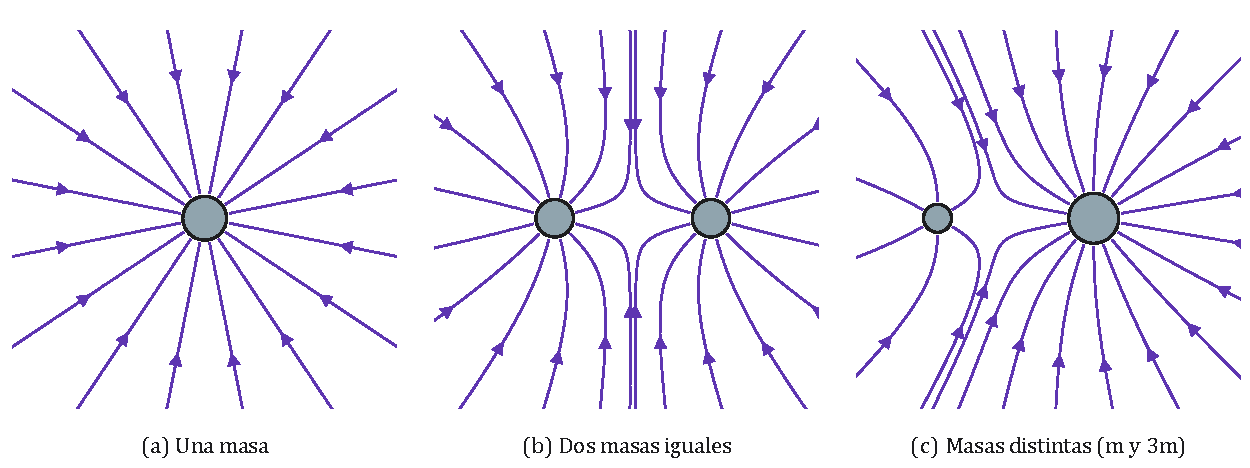
\includegraphics[width=0.95\linewidth]{images/UD4/lineas_campo}
    \caption{Líneas del campo gravitatorio (calculadas con la ley de Newton). En (b), en el punto medio el campo es nulo;
    en (c), a la masa mayor llegan tres veces más líneas.}
    \label{fig:grav-lineas}
\end{figure}

\subsection{El campo gravitatorio terrestre}\label{subsec:grav-terrestre}

Fuera de ella, la Tierra crea el mismo campo que si toda su masa estuviera en su centro. En la superficie:
\begin{centeredequation}
    \boxed{g_0 = G\,\dfrac{M_T}{R_T^2}} = 6{,}67\cdot 10^{-11}\,\dfrac{5{,}98\cdot 10^{24}}{(6{,}37\cdot 10^6)^2} \approx \qty{9.8}{\newton\per\kg} \label{eq:grav-g0}
\end{centeredequation}
De aquí sale una relación muy útil: \(\boxed{G M_T = g_0 R_T^2}\), que permite resolver muchos problemas sin conocer \(G\) ni
\(M_T\).

\paragraph{Variación con la altura.} A una altura \(h\):
\begin{centeredequation}
    g = G\,\dfrac{M_T}{(R_T + h)^2} = g_0\,\dfrac{R_T^2}{(R_T + h)^2} \label{eq:grav-g-altura}
\end{centeredequation}

\paragraph{Variación con la profundidad.} Dentro de la Tierra, a una distancia \(r = R_T - h\) del centro, solo atrae la
masa de la esfera de radio \(r\) (la capa exterior no produce campo neto). Suponiendo la densidad \(\rho\) uniforme, esa masa
es \(m = \rho\,\tfrac{4}{3}\pi r^3\) y \(M_T = \rho\,\tfrac{4}{3}\pi R_T^3\):
\begin{equation*}
    \dfrac{g_h}{g_0} = \dfrac{G m/r^2}{G M_T/R_T^2} = \dfrac{r^3 R_T^2}{R_T^3 r^2} = \dfrac{r}{R_T}
    \qquad\Rightarrow\qquad \boxed{g_h = g_0\,\dfrac{R_T - h}{R_T}}
\end{equation*}
Dentro de la Tierra, \(g\) crece linealmente desde cero en el centro; fuera, disminuye con \(1/r^2\)
(figuras~\ref{fig:grav-profundidad} y \ref{fig:grav-g-r}).

\begin{figure}[H]
    \centering
    \begin{minipage}[b]{0.38\linewidth}
        \centering
        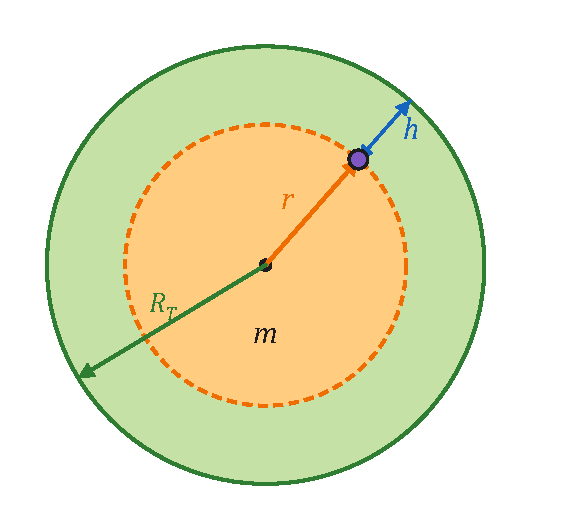
\includegraphics[width=\linewidth]{images/UD4/profundidad}
        \caption{A una profundidad \(h\) solo atrae la esfera interior de radio \(r\).}
        \label{fig:grav-profundidad}
    \end{minipage}\hfill
    \begin{minipage}[b]{0.56\linewidth}
        \centering
        \begin{tikzpicture}
            \begin{axis}[fisica, width=\linewidth, height=5cm, xmin=0, xmax=4.3, ymin=0, ymax=1.25,
                xlabel={\(r\)}, ylabel={\(g\)}, xtick={1,2,3,4}, xticklabels={\(R_T\),\(2R_T\),\(3R_T\),\(4R_T\)},
                ytick={1}, yticklabels={\(g_0\)}]
                \addplot[domain=0:1, very thick, ocre] {x};
                \addplot[domain=1:4.1, very thick, ocre] {1/x^2};
                \draw[dashed, gray] (axis cs:1,0) -- (axis cs:1,1);
            \end{axis}
        \end{tikzpicture}
        \caption{Intensidad del campo terrestre en función de la distancia al centro.}
        \label{fig:grav-g-r}
    \end{minipage}
\end{figure}

\paragraph{Peso.} El \rojon{peso} de un cuerpo es la fuerza con que lo atrae la Tierra: \(P = m\,g\), un vector dirigido
hacia el centro de la Tierra cuyo módulo depende de la altura (y de la latitud). La masa, en cambio, es la misma en
cualquier lugar.

\begin{exercise}
    ¿Cuánto vale el campo gravitatorio creado por un cuerpo de \qty{500}{\kg} a \qty{5}{\m} de su centro?
    \begin{solu}
        \(g = G\,\dfrac{M}{r^2} = 6{,}67\cdot 10^{-11}\cdot\dfrac{500}{25} = \textcolor{red}{\qty{1.33e-9}{\newton\per\kg}}\): \textcolor{blue}{insignificante.}
    \end{solu}
\end{exercise}

\begin{exercise}
    ¿A qué distancia de un cuerpo de masa \(4m\) el campo vale lo mismo que a una distancia \(r\) de un cuerpo de masa \(m\)?
    \begin{solu}
        \(G\,\dfrac{4m}{r'^2} = G\,\dfrac{m}{r^2} \Rightarrow r'^2 = 4r^2 \Rightarrow \textcolor{red}{r' = 2r}\).
    \end{solu}
\end{exercise}

\begin{exercise}
    ¿A qué altura hay que subir para que la intensidad del campo terrestre disminuya un \qty{19}{\percent}? ¿Y para que el
    peso de una persona se reduzca al \qty{64}{\percent}? (\(R_T = \qty{6370}{\km}\)).
    \begin{solu}
        \textcolor{blue}{\(\dfrac{g}{g_0} = \dfrac{R_T^2}{(R_T + h)^2} \Rightarrow R_T + h = R_T\sqrt{g_0/g}\).}

        \(g = 0{,}81\,g_0\): \(R_T + h = \dfrac{R_T}{0{,}9} \Rightarrow h = \dfrac{R_T}{9} = \textcolor{red}{\qty{708}{\km}}\).

        \(P = 0{,}64\,P_0\): \(R_T + h = \dfrac{R_T}{0{,}8} \Rightarrow h = \dfrac{R_T}{4} = \textcolor{red}{\qty{1592}{\km}}\).
    \end{solu}
\end{exercise}

\begin{exercise}
    Júpiter tiene una densidad media de \qty{1.33}{\g\per\cm\cubed} y un radio de \qty{6.99e4}{\km}. Calcula la intensidad del
    campo gravitatorio en su superficie.
    \begin{solu}
        \textcolor{blue}{\(M = \rho\,\tfrac{4}{3}\pi R^3\), así que \(g = G\,\dfrac{M}{R^2} = \tfrac{4}{3}\pi G\rho R\):}
        \[ g = \tfrac{4}{3}\pi\cdot 6{,}67\cdot 10^{-11}\cdot 1330\cdot 6{,}99\cdot 10^7 = \textcolor{red}{\qty{26.0}{\newton\per\kg}} \]
    \end{solu}
\end{exercise}

\section{Energía potencial gravitatoria}\label{sec:grav-energia}

\subsection{La fuerza gravitatoria es conservativa}\label{subsec:grav-conservativa}

Calculemos el trabajo que hace la fuerza gravitatoria de una masa \(M\) sobre otra \(m\) que va de \(A\) a \(B\) por dos
caminos formados por tramos radiales y arcos de circunferencia centrados en \(M\) (figura~\ref{fig:grav-trabajo}). En los
arcos la fuerza es perpendicular al desplazamiento y no trabaja; en los tramos radiales, \(\vec F\) y \(d\vec r\) son
opuestos:
\begin{equation*}
    W_{A\to B} = \int_{r_A}^{r_B} -\,G\,\dfrac{M m}{r^2}\,dr = G M m\left[\dfrac{1}{r}\right]_{r_A}^{r_B} = \dfrac{G M m}{r_B} - \dfrac{G M m}{r_A}
\end{equation*}
Por los dos caminos sale lo mismo, y cualquier camino se puede aproximar por pequeños tramos radiales y arcos. El trabajo
\textbf{no depende de la trayectoria}, solo de las posiciones inicial y final; y en una trayectoria cerrada es nulo. La
fuerza gravitatoria es \rojon{conservativa}, como todas las fuerzas centrales.

\begin{figure}[H]
    \centering
    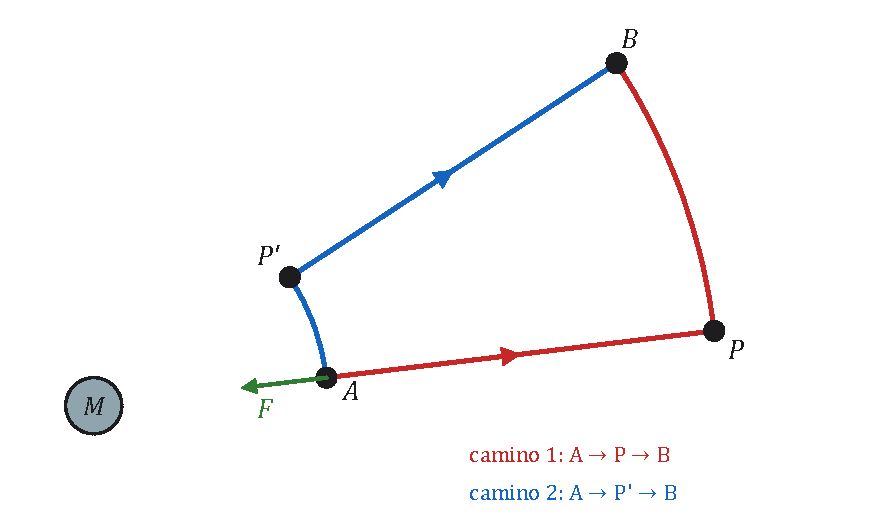
\includegraphics[width=0.55\linewidth]{images/UD4/trabajo_conservativo}
    \caption{El trabajo de la fuerza gravitatoria de \(A\) a \(B\) es el mismo por los dos caminos.}
    \label{fig:grav-trabajo}
\end{figure}

\subsection{Energía potencial}\label{subsec:grav-ep}

Para una fuerza conservativa se puede definir una energía potencial tal que \(W_{A\to B} = -\Delta E_p = E_{p,A} - E_{p,B}\).
Comparando con el trabajo calculado, y tomando \(E_p = 0\) en el infinito:
\begin{centeredequation}
    \boxed{E_p = -\,G\,\dfrac{M m}{r}} \label{eq:grav-ep}
\end{centeredequation}
La energía potencial de dos masas separadas una distancia \(r\) es el trabajo que hace la fuerza gravitatoria cuando se
separan hasta el infinito. Es \textbf{siempre negativa} y aumenta (se hace menos negativa) al alejarse: hay que hacer un
trabajo contra el campo para separarlas. Es una magnitud escalar que se mide en julios. Si hay más de dos masas, la energía
potencial del sistema es la suma de las energías de cada pareja.

\begin{figure}[H]
    \centering
    \begin{tikzpicture}
        \begin{axis}[fisica, width=0.55\linewidth, height=4.6cm, xmin=0, xmax=5.3, ymin=-1.15, ymax=0.25,
            xlabel={\(r\)}, ylabel={\(E_p\)}, xtick=\empty, ytick=\empty, axis x line=middle]
            \addplot[domain=0.9:5, very thick, ocre] {-1/x};
        \end{axis}
    \end{tikzpicture}
    \caption{La energía potencial gravitatoria es negativa y tiende a cero en el infinito.}
    \label{fig:grav-ep}
\end{figure}

\paragraph{Cerca de la superficie: \(E_p = mgh\).} Al subir un cuerpo desde la superficie hasta una altura \(h\):
\begin{equation*}
    \Delta E_p = -\dfrac{G M_T m}{R_T + h} + \dfrac{G M_T m}{R_T} = G M_T m\,\dfrac{h}{R_T(R_T + h)} = m\,g_0\,\dfrac{R_T\,h}{R_T + h}
\end{equation*}
Si \(h \ll R_T\), \(R_T + h \approx R_T\) y queda \(\Delta E_p = m g_0 h\), la expresión que se usa en los cursos anteriores.
Para alturas grandes hay que usar la expresión general.

\begin{exercise}
    Dos partículas de \qty{3}{\kg} y \qty{5}{\kg} están separadas \qty{30}{\cm}. Calcula la energía potencial del sistema, el
    trabajo de la fuerza gravitatoria al separarlas hasta \qty{90}{\cm} y el trabajo para llevar una de ellas al infinito.
    \begin{solu}
        \(E_{p,1} = -G\,\dfrac{3\cdot 5}{0{,}3} = \textcolor{red}{\qty{-3.34e-9}{\joule}}\); \(E_{p,2} = -G\,\dfrac{15}{0{,}9} = \qty{-1.11e-9}{\joule}\).

        \(W = -\Delta E_p = E_{p,1} - E_{p,2} = \textcolor{red}{\qty{-2.22e-9}{\joule}}\);
        \(W_{\to\infty} = E_{p,1} - 0 = \textcolor{red}{\qty{-3.34e-9}{\joule}}\).
        \textcolor{blue}{Son negativos: la gravedad se opone a la separación.}
    \end{solu}
\end{exercise}

\begin{exercise}
    ¿Cuál es la energía potencial de un satélite de \qty{5000}{\kg} que orbita a \qty{600}{\km} de altura?
    (\(M_T = \qty{5.98e24}{\kg}\), \(R_T = \qty{6370}{\km}\)).
    \begin{solu}
        \(E_p = -\dfrac{G M_T m}{R_T + h} = -\dfrac{6{,}67\cdot 10^{-11}\cdot 5{,}98\cdot 10^{24}\cdot 5000}{6{,}97\cdot 10^6} = \textcolor{red}{\qty{-2.86e11}{\joule}}\).
    \end{solu}
\end{exercise}

\begin{exercise}
    Calcula la energía potencial del sistema formado por tres masas de \qty{3}{\kg}, \qty{5}{\kg} y \qty{4}{\kg} situadas en
    \((0, 0)\), \((0, 4)\) y \((3, 0)\) (en metros).
    \begin{solu}
        \textcolor{blue}{Distancias: \(r_{12} = 4\), \(r_{13} = 3\), \(r_{23} = 5\) m.}
        \[ E_p = -G\left(\dfrac{3\cdot 5}{4} + \dfrac{3\cdot 4}{3} + \dfrac{5\cdot 4}{5}\right) = -6{,}67\cdot 10^{-11}\cdot 11{,}75 = \textcolor{red}{\qty{-7.84e-10}{\joule}} \]
    \end{solu}
\end{exercise}

\section{Potencial gravitatorio}\label{sec:grav-potencial}

\begin{definition}[Potencial gravitatorio]
    El \rojon{potencial gravitatorio} \(V\) en un punto es la energía potencial por unidad de masa colocada en él:
    \(V = E_p/m\). Para una masa puntual \(M\):
    \begin{centeredequation}
        \boxed{V = -\,G\,\dfrac{M}{r}} \label{eq:grav-V}
    \end{centeredequation}
    Es un escalar, se mide en \unit{\joule\per\kg} y es nulo en el infinito. El potencial creado por varias masas es la suma
    (escalar) de los potenciales de cada una.
\end{definition}

\paragraph{Diferencia de potencial y trabajo.} Como \(W = -\Delta E_p\) y \(E_p = mV\), el trabajo que hace el campo al
llevar una masa \(m\) de \(A\) a \(B\) es:
\begin{centeredequation}
    \boxed{W_{A\to B} = -\,m\,(V_B - V_A) = m\,(V_A - V_B)} \label{eq:grav-trabajo-V}
\end{centeredequation}
Si \(W > 0\), el desplazamiento es espontáneo (la masa va hacia potenciales menores); si \(W < 0\), hay que aportar energía.

\paragraph{Superficies equipotenciales.} Son los lugares geométricos de los puntos con el mismo potencial. Para una masa
puntual son esferas centradas en ella. Las líneas de campo son siempre \textbf{perpendiculares} a las superficies
equipotenciales, y mover una masa sobre una equipotencial no cuesta trabajo (figura~\ref{fig:grav-equipotenciales}).

\begin{figure}[H]
    \centering
    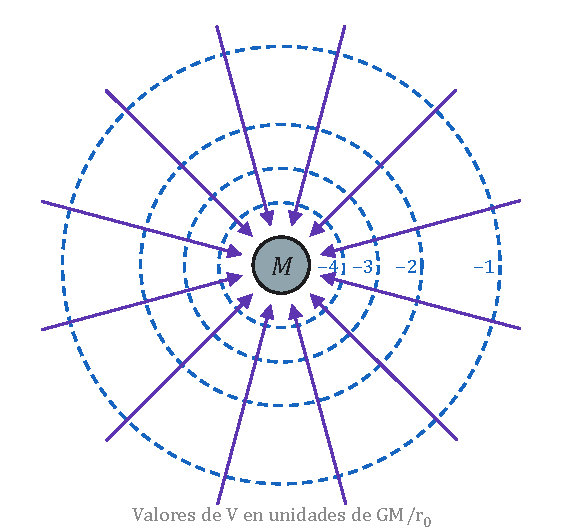
\includegraphics[width=0.42\linewidth]{images/UD4/equipotenciales}
    \caption{Superficies equipotenciales (en discontinuo) y líneas de campo de una masa puntual.}
    \label{fig:grav-equipotenciales}
\end{figure}

\begin{exercise}
    Dos masas de \qty{5}{\kg} están en \((0, 0)\) y \((8, 0)\) (en metros). Calcula el trabajo que hace el campo al llevar una
    masa de \qty{1}{\kg} desde el punto \((4, 3)\) hasta el \((4, 0)\).
    \begin{solu}
        \textcolor{blue}{En \(A(4, 3)\) cada masa está a \qty{5}{\m}; en \(B(4, 0)\), a \qty{4}{\m}.}
        \[ V_A = -2\,G\,\dfrac{5}{5} = \qty{-1.334e-10}{\joule\per\kg} \qquad V_B = -2\,G\,\dfrac{5}{4} = \qty{-1.668e-10}{\joule\per\kg} \]
        \(W = m(V_A - V_B) = \textcolor{red}{\qty{3.34e-11}{\joule}}\) \textcolor{blue}{(positivo: el campo lo hace solo).}
    \end{solu}
\end{exercise}

\section{Movimiento de planetas y satélites}\label{sec:grav-satelites}

\subsection{Velocidad orbital y período}\label{subsec:grav-orbital}

Un satélite de masa \(m\) en órbita circular de radio \(r = R + h\) alrededor de un planeta de masa \(M\) y radio \(R\) está
sometido solo a la atracción gravitatoria, que hace de fuerza centrípeta (figura~\ref{fig:grav-satelite}):
\begin{equation*}
    G\,\dfrac{M m}{r^2} = m\,\dfrac{v^2}{r} \qquad\Rightarrow\qquad \boxed{v = \sqrt{\dfrac{G M}{r}}} \qquad\qquad \boxed{T = \dfrac{2\pi r}{v} = 2\pi\sqrt{\dfrac{r^3}{G M}}}
\end{equation*}
La velocidad orbital no depende de la masa del satélite y es menor cuanto más alta es la órbita.

\begin{figure}[H]
    \centering
    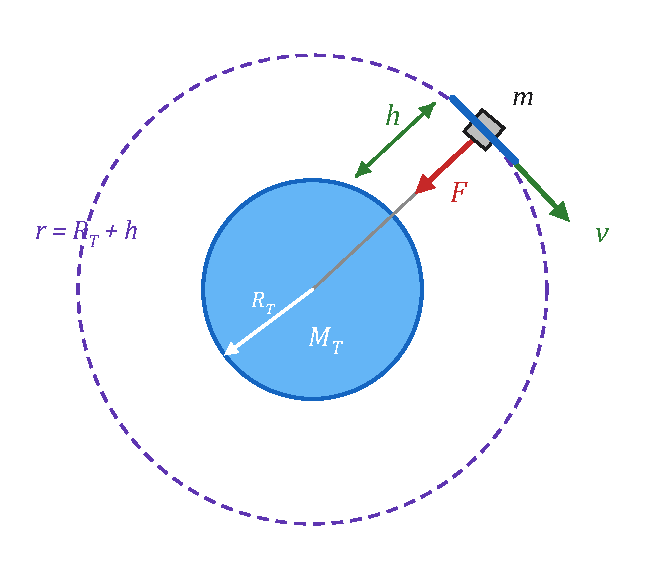
\includegraphics[width=0.45\linewidth]{images/UD4/satelite}
    \caption{Satélite en órbita circular a una altura \(h\).}
    \label{fig:grav-satelite}
\end{figure}

\paragraph{Satélites geoestacionarios.} Si el período de un satélite es igual al de rotación de la Tierra (un día sidéreo,
\qty{86164}{\second}) y gira en el plano del ecuador, en el mismo sentido que la Tierra, está siempre sobre el mismo punto de
la superficie. Se usan para comunicaciones y televisión.

\subsection{Energía de un satélite en órbita}\label{subsec:grav-energia-satelite}

Con \(v^2 = G M/r\):
\begin{equation*}
    E_c = \dfrac{1}{2} m v^2 = \dfrac{G M m}{2r} \qquad\qquad E_p = -\,\dfrac{G M m}{r}
\end{equation*}
\begin{centeredequation}
    \boxed{E_m = E_c + E_p = -\,\dfrac{G M m}{2r}} \qquad\qquad E_c = -E_m = -\tfrac{1}{2}E_p \label{eq:grav-em-orbita}
\end{centeredequation}
La energía mecánica de un satélite en órbita es negativa: está \emph{ligado} al planeta. Si solo actúa la gravedad, la
energía mecánica se conserva: \(\tfrac{1}{2}m v_1^2 - \dfrac{GMm}{r_1} = \tfrac{1}{2}m v_2^2 - \dfrac{GMm}{r_2}\).

\paragraph{Energía para poner un satélite en órbita.} Desde la superficie (despreciando la rotación de la Tierra y el
rozamiento), la energía que hay que comunicar es la diferencia entre la energía mecánica en la órbita y la energía potencial
en la superficie:
\begin{equation*}
    \Delta E = -\,\dfrac{G M m}{2r} - \left(-\,\dfrac{G M m}{R}\right) = G M m\left(\dfrac{1}{R} - \dfrac{1}{2r}\right)
\end{equation*}

\paragraph{Energía para cambiar de órbita.} Para pasar de una órbita de radio \(r_1\) a otra de radio \(r_2\):
\(\Delta E = E_{m,2} - E_{m,1} = \dfrac{G M m}{2}\left(\dfrac{1}{r_1} - \dfrac{1}{r_2}\right)\).

\begin{exercise}
    Un meteorito de \qty{500}{\kg} está en reposo a una altura igual a tres veces el radio terrestre. Si cae sin rozamiento,
    ¿con qué velocidad llega a la superficie? (\(M_T = \qty{5.98e24}{\kg}\), \(R_T = \qty{6370}{\km}\)).
    \begin{solu}
        \textcolor{blue}{Parte de \(r_1 = 4R_T\) con \(v_1 = 0\). Conservación de la energía:}
        \[ -\dfrac{G M_T m}{4R_T} = \dfrac{1}{2}m v^2 - \dfrac{G M_T m}{R_T} \;\Rightarrow\; v = \sqrt{2 G M_T\left(\dfrac{1}{R_T} - \dfrac{1}{4R_T}\right)} = \sqrt{\dfrac{3 G M_T}{2 R_T}} = \textcolor{red}{\qty{9.69e3}{\m\per\second}} \]
        \textcolor{blue}{(No depende de la masa del meteorito.)}
    \end{solu}
\end{exercise}

\begin{exercise}
    Se quiere poner en órbita circular de \qty{7500}{\km} de radio un satélite de \qty{800}{\kg} lanzado desde la superficie
    terrestre. ¿Qué energía hay que comunicarle? Si después se pasa a una órbita de \qty{9000}{\km} de radio, ¿cuánta energía
    hace falta? (\(M_T = \qty{5.98e24}{\kg}\), \(R_T = \qty{6370}{\km}\)).
    \begin{solu}
        \(\Delta E_1 = G M_T m\left(\dfrac{1}{R_T} - \dfrac{1}{2r_1}\right) = 3{,}19\cdot 10^{17}\left(\dfrac{1}{6{,}37\cdot 10^6} - \dfrac{1}{1{,}5\cdot 10^7}\right) = \textcolor{red}{\qty{2.88e10}{\joule}}\).

        \(\Delta E_2 = \dfrac{G M_T m}{2}\left(\dfrac{1}{r_1} - \dfrac{1}{r_2}\right) = \textcolor{red}{\qty{3.55e9}{\joule}}\).
    \end{solu}
\end{exercise}

\subsection{Velocidad de escape}\label{subsec:grav-escape}

\begin{definition}[Velocidad de escape]
    La \rojon{velocidad de escape} es la velocidad mínima que hay que comunicar a un cuerpo en la superficie de un astro
    para que escape de su atracción, es decir, para que llegue al infinito (\(E_p = 0\)) con velocidad nula (\(E_c = 0\)).
\end{definition}
Por la conservación de la energía:
\begin{equation*}
    \dfrac{1}{2}m v_e^2 - \dfrac{G M m}{R} = 0 + 0 \qquad\Rightarrow\qquad \boxed{v_e = \sqrt{\dfrac{2 G M}{R}} = \sqrt{2 g_0 R}}
\end{equation*}
No depende de la masa del cuerpo. Para la Tierra vale unos \qty{11.2}{\km\per\second} y para la Luna, \qty{2.4}{\km\per\second}.
Un cuerpo lanzado con la velocidad de escape tiene energía mecánica nula; si la supera, su energía es positiva y no vuelve.

\begin{remark}
    Según su energía mecánica, un cuerpo en el campo de un astro: si \(E_m < 0\), está ligado y describe una órbita cerrada
    (circular o elíptica); si \(E_m = 0\), escapa justo (trayectoria parabólica); si \(E_m > 0\), escapa con velocidad sobrante
    (trayectoria hiperbólica).
\end{remark}

\section{Resumen de fórmulas}\label{sec:grav-resumen}

\begin{table}[H]
    \centering
    \caption{Fórmulas principales de la interacción gravitatoria}
    \vspace{-5pt}
    \begin{tabular}{@{}lL{10cm}@{}}
        \toprule
        \textbf{Magnitud} & \textbf{Expresión} \\
        \midrule
        Tercera ley de Kepler & \(T^2/r^3 = 4\pi^2/(GM)\) \\[3pt]
        Momento angular & \(\vec L = \vec r\times m\vec v\); \quad fuerza central: \(\vec L\) constante, \(r_p v_p = r_a v_a\) \\[3pt]
        Gravitación universal & \(F = G\,m_1 m_2/r^2\), \quad \(G = \qty{6.67e-11}{\newton\m\squared\per\kg\squared}\) \\[3pt]
        Campo gravitatorio & \(g = GM/r^2\), \quad \(\vec F = m\vec g\), \quad \(G M_T = g_0 R_T^2\) \\[3pt]
        Campo dentro de la Tierra & \(g_h = g_0\,(R_T - h)/R_T\) \\[3pt]
        Energía potencial & \(E_p = -\,GMm/r\) \quad (cerca de la superficie, \(\Delta E_p = mgh\)) \\[3pt]
        Potencial & \(V = -\,GM/r\), \quad \(W_{A\to B} = m(V_A - V_B)\) \\[3pt]
        Satélite en órbita & \(v = \sqrt{GM/r}\), \quad \(T = 2\pi\sqrt{r^3/GM}\), \quad \(E_m = -\,GMm/(2r)\) \\[3pt]
        Velocidad de escape & \(v_e = \sqrt{2GM/R} = \sqrt{2 g_0 R}\) \\
        \bottomrule
    \end{tabular}
    \label{tab:grav-resumen}
\end{table}

\section{Prácticas}\label{sec:grav-practicas}

\subsection{Práctica 1: la tercera ley de Kepler con las lunas de Júpiter}\label{subsec:grav-practica-kepler}

\textbf{Objetivo.} Comprobar la tercera ley de Kepler con los satélites galileanos de Júpiter y calcular la masa del planeta.

\textbf{Material.} Datos de la tabla (o medidas propias hechas con un telescopio pequeño o con un programa planetario
gratuito, siguiendo varias noches la posición de las lunas), hoja de cálculo.

\begin{table}[H]
    \centering
    \caption{Satélites galileanos de Júpiter}
    \vspace{-5pt}
    \begin{tabular}{@{}lcccc@{}}
        \toprule
        \textbf{Satélite} & \textbf{\(r\) (\(10^8\) \unit{\m})} & \textbf{\(T\) (días)} & \textbf{\(r^3\) (\unit{\m\cubed})} & \textbf{\(T^2\) (\unit{\second\squared})} \\
        \midrule
        Ío & \num{4.22} & \num{1.769} & & \\[3pt]
        Europa & \num{6.71} & \num{3.551} & & \\[3pt]
        Ganímedes & \num{10.70} & \num{7.155} & & \\[3pt]
        Calisto & \num{18.83} & \num{16.69} & & \\
        \bottomrule
    \end{tabular}
    \label{tab:grav-practica-kepler}
\end{table}

\textbf{Procedimiento.}
\begin{enumerate}[label=\numberballmDarkTeal]
    \item Pasa los radios a metros y los períodos a segundos y completa la tabla.
    \item Representa \(T^2\) frente a \(r^3\). Comprueba que los puntos están sobre una recta que pasa por el origen.
    \item Calcula la pendiente de la recta, \(k = T^2/r^3\).
\end{enumerate}

\textbf{Cálculos y cuestiones.}
\begin{enumerate}[label=\letraminuscula]
    \item Como \(k = 4\pi^2/(G M_J)\), calcula la masa de Júpiter. (Valor aceptado: \qty{1.90e27}{\kg}.)
    \item ¿Por qué la recta debe pasar por el origen?
    \item Busca los datos de cuatro planetas del Sistema Solar, haz la misma gráfica y calcula la masa del Sol.
\end{enumerate}

\subsection{Práctica 2: medida de \texorpdfstring{\(g\)}{g} y de la masa de la Tierra}\label{subsec:grav-practica-g}

\textbf{Objetivo.} Medir la aceleración de la gravedad y, a partir de ella, estimar la masa y la densidad media de la Tierra.

\textbf{Material.} Péndulo simple (hilo y bola), cronómetro y regla (la práctica 2 de la unidad 1); o bien un teléfono
móvil con una aplicación que registre el acelerómetro.

\textbf{Procedimiento.}
\begin{enumerate}[label=\numberballmDarkTeal]
    \item Mide \(g\) con el péndulo (\(g = 4\pi^2 l/T^2\)) para varias longitudes y halla el valor medio.
    \item Alternativa: deja el móvil quieto sobre la mesa y anota la aceleración que marca el sensor en el eje vertical.
\end{enumerate}

\textbf{Cálculos y cuestiones.}
\begin{enumerate}[label=\letraminuscula]
    \item Con \(G M_T = g_0 R_T^2\) y \(R_T = \qty{6370}{\km}\), calcula la masa de la Tierra.
    \item Calcula su densidad media y compárala con la de las rocas de la superficie (unos \qty{2.7}{\g\per\cm\cubed}).
    ¿Qué te dice sobre el interior de la Tierra?
    \item ¿Cuánto debería cambiar \(g\) al subir al último piso del instituto (unos \qty{15}{\m})? ¿Podrías medir esa diferencia
    con tu montaje?
\end{enumerate}
